\documentclass[nooutcomes]{ximera}


\graphicspath{
  {./}
  {1-1QuantitativeReasoning/}
  {1-2RelationsAndGraphs/}
  {1-3ChangingInTandem/}
  {2-1LinearEquations/}
  {2-2LinearModeling/}
  {2-3ExponentialModeling/}
  {3-1WhatIsAFunction/}
  {3-2FunctionProperties/}
  {3-3AverageRatesOfChange/}
  {4-1BuildingNewFunctions/}
  {4-2Polynomials/}
  {5-1RationalFunctions/}
   {5-2ExponentialFunctions/}
  {6-1Domain/}
  {6-2Range/}
  {6-3CompositionOfFunctions/}
  {7-1ZerosOfFunctions/}
  {7-XZerosOfPolynomials/}
  {7-2ZerosOfFamousFunctions/}
  {8-0Review/}
  {8-1FunctionTransformations/}
  {8-2SolvingInequalities/}
  {8-3FunctionTransformationsProject/}
  {9-1RightTriangleTrig/}
  {9-2TheUnitCircle/}
  {9-3TrigIdentities/}
  {10-1UnitCircleToFunctionGraph/}
  {10-2TrigFunctions/}
  {10-3SomeApplicationsOfTrig/}
  {11-1InverseFunctionsRevisited/}
  {11-2Logarithms/}
  {11-3InverseTrig/}
  {12-1SystemsOfEquations/}
  {12-2NonlinearSystems/}
  {12-3ApplicationsOfSystems/}
  {13-1SecantLinesRevisited/}
  {13-2Functions-TheBigPicture/}
  {14-1DisplacementVsDistance/}
  {1-1QuantitativeReasoning/exercises/}
  {1-2RelationsAndGraphs/exercises/}
  {../1-3ChangingInTandem/exercises/}
  {../2-1LinearEquations/exercises/}
  {../2-2LinearModeling/exercises/}
  {../2-3ExponentialModeling/exercises/}
  {../3-1WhatIsAFunction/exercises/}
  {../3-2FunctionProperties/exercises/}
  {../3-3AverageRatesOfChange/exercises/}
  {../5-2ExponentialFunctions/exercises/}
  {../4-1BuildingNewFunctions/exercises/}
  {../4-2Polynomials/exercises/}
  {../5-1RationalFunctions/exercises/}
  {../6-1Domain/exercises/}
  {../6-2Range/exercises/}
  {../6-3CompositionOfFunctions/exercises/}
  {../7-1ZerosOfFunctions/exercises/}
  {../7-XZerosOfPolynomials/exercises/}
  {../7-2ZerosOfFamousFunctions/exercises/}
  {../8-1FunctionTransformations/exercises/}
  {../12-1SystemsOfEquations/exercises/}
  {../8-3FunctionTransformationsProject/exercises/}
  {../8-0Review/exercises/}
  {../8-2SolvingInequalities/exercises/}
  {../8-3FunctionTransformationsProject/exercises/}
  {../9-1RightTriangleTrig/exercises/}
  {../9-2TheUnitCircle/exercises/}
  {../9-3TrigIdentities/exercises/}
  {../10-1UnitCircleToFunctionGraph/exercises/}
  {../10-2TrigFunctions/exercises/}
  {../10-3SomeApplicationsOfTrig/exercises/}
  {../11-1InverseFunctionsRevisited/exercises/}
  {../11-2Logarithms/exercises/}
  {../11-3InverseTrig/exercises/}
  {../12-1SystemsOfEquations/exercises/}
  {../12-2NonlinearSystems/exercises/}
  {../12-3ApplicationsOfSystems/exercises/}
  {../13-1SecantLinesRevisited/exercises/}
  {../13-2Functions-TheBigPicture/exercises/}
  {../14-1DisplacementVsDistance/exercises/}
}

\DeclareGraphicsExtensions{.pdf,.png,.jpg,.eps}

\newcommand{\mooculus}{\textsf{\textbf{MOOC}\textnormal{\textsf{ULUS}}}}

\usepackage[makeroom]{cancel} %% for strike outs

\ifxake
\else
\usepackage[most]{tcolorbox}
\fi


%\typeout{************************************************}
%\typeout{New Environments}
%\typeout{************************************************}

%% to fix for web can be removed when deployed offically with ximera2
\let\image\relax\let\endimage\relax
\NewEnviron{image}{% 
  \begin{center}\BODY\end{center}% center
}



\NewEnviron{folder}{
      \addcontentsline{toc}{section}{\textbf{\BODY}}
}

\ifxake
\let\summary\relax
\let\endsummary\relax
\newtheorem*{summary}{Summary}
\newtheorem*{callout}{Callout}
\newtheorem*{overview}{Overview}
\newtheorem*{objectives}{Objectives}
\newtheorem*{motivatingQuestions}{Motivating Questions}
\newtheorem*{MM}{Metacognitive Moment}
      
%% NEEDED FOR XIMERA 2
%\ximerizedEnvironment{summary}
%\ximerizedEnvironment{callout}
%\ximerizedEnvironment{overview} 
%\ximerizedEnvironment{objectives}
%\ximerizedEnvironment{motivatingQuestions}
%\ximerizedEnvironment{MM}
\else
%% CALLOUT
\NewEnviron{callout}{
  \begin{tcolorbox}[colback=blue!5, breakable,pad at break*=1mm]
      \BODY
  \end{tcolorbox}
}
%% MOTIVATING QUESTIONS
\NewEnviron{motivatingQuestions}{
  \begin{tcolorbox}[ breakable,pad at break*=1mm]
    \textbf{\Large Motivating Questions}\hfill
    %\begin{itemize}[label=\textbullet]
      \BODY
    %\end{itemize}
  \end{tcolorbox}
}
%% OBJECTIVES
\NewEnviron{objectives}{  
    \vspace{.5in}
      %\begin{tcolorbox}[colback=orange!5, breakable,pad at break*=1mm]
    \textbf{\Large Learning Objectives}
    \begin{itemize}[label=\textbullet]
      \BODY
    \end{itemize}
    %\end{tcolorbox}
}
%% DEFINITION
\let\definition\relax
\let\enddefinition\relax
\NewEnviron{definition}{
  \begin{tcolorbox}[ breakable,pad at break*=1mm]
    \noindent\textbf{Definition}~
      \BODY
  \end{tcolorbox}
}
%% OVERVIEW
\let\overview\relax
\let\overview\relax
\NewEnviron{overview}{
  \begin{tcolorbox}[ breakable,pad at break*=1mm]
    \textbf{\Large Overview}
    %\begin{itemize}[label=\textbullet] %% breaks Xake
      \BODY
    %\end{itemize}
  \end{tcolorbox}
}
%% SUMMARY
\let\summary\relax
\let\endsummary\relax
\NewEnviron{summary}{
  \begin{tcolorbox}[ breakable,pad at break*=1mm]
    \textbf{\Large Summary}
    %\begin{itemize}[label=\textbullet] %% breaks Xake
      \BODY
    %\end{itemize}
  \end{tcolorbox}
}
%% REMARK
\let\remark\relax
\let\endremark\relax
\NewEnviron{remark}{
  \begin{tcolorbox}[colback=green!5, breakable,pad at break*=1mm]
    \noindent\textbf{Remark}~
      \BODY
  \end{tcolorbox}
}
%% EXPLANATION
\let\explanation\relax
\let\endexplanation\relax
\NewEnviron{explanation}{
    \normalfont
    \noindent\textbf{Explanation}~
      \BODY
}
%% EXPLORATION
\let\exploration\relax
\let\endexploration\relax
\NewEnviron{exploration}{
  \begin{tcolorbox}[colback=yellow!10, breakable,pad at break*=1mm]
    \noindent\textbf{Exploration}~
      \BODY
  \end{tcolorbox}
}
%% METACOGNITIVE MOMENTS
\let\MM\relax
\let\endMM\relax
\NewEnviron{MM}{
  \begin{tcolorbox}[colback=pink!15, breakable,pad at break*=1mm]
    \noindent\textbf{Metacognitive Moment}~
      \BODY
  \end{tcolorbox}
}


\fi





%Notes on what envirnoment to use:  Example with Explanation in text; if they are supposed to answer- Problem; no answer - Exploration


%\typeout{************************************************}
%% Header and footers
%\typeout{************************************************}

\newcommand{\licenseAcknowledgement}{Licensed under Creative Commons 4.0}
\newcommand{\licenseAPC}{\renewcommand{\licenseAcknowledgement}{\textbf{Acknowledgements:} Active Prelude to Calculus (https://activecalculus.org/prelude) }}
\newcommand{\licenseSZ}{\renewcommand{\licenseAcknowledgement}{\textbf{Acknowledgements:} Stitz Zeager Open Source Mathematics (https://www.stitz-zeager.com/) }}
\newcommand{\licenseAPCSZ}{\renewcommand{\licenseAcknowledgement}{\textbf{Acknowledgements:} Active Prelude to Calculus (https://activecalculus.org/prelude) and Stitz Zeager Open Source Mathematics (https://www.stitz-zeager.com/) }}
\newcommand{\licenseORCCA}{\renewcommand{\licenseAcknowledgement}{\textbf{Acknowledgements:}Original source material, products with readable and accessible
math content, and other information freely available at pcc.edu/orcca.}}
\newcommand{\licenseY}{\renewcommand{\licenseAcknowledgement}{\textbf{Acknowledgements:} Yoshiwara Books (https://yoshiwarabooks.org/)}}
\newcommand{\licenseOS}{\renewcommand{\licenseAcknowledgement}{\textbf{Acknowledgements:} OpenStax College Algebra (https://openstax.org/details/books/college-algebra)}}
\newcommand{\licenseAPCSZCSCC}{\renewcommand{\licenseAcknowledgement}{\textbf{Acknowledgements:} Active Prelude to Calculus (https://activecalculus.org/prelude), Stitz Zeager Open Source Mathematics (https://www.stitz-zeager.com/), CSCC PreCalculus and Calculus texts (https://ximera.osu.edu/csccmathematics)}}

\ifxake\else %% do nothing on the website
\usepackage{fancyhdr}
\pagestyle{fancy}
\fancyhf{}
\fancyhead[R]{\sectionmark}
\fancyfoot[L]{\thepage}
\fancyfoot[C]{\licenseAcknowledgement}
\renewcommand{\headrulewidth}{0pt}
\renewcommand{\footrulewidth}{0pt}
\fi

%%%%%%%%%%%%%%%%



%\typeout{************************************************}
%\typeout{Table of Contents}
%\typeout{************************************************}


%% Edit this to change the font style
\newcommand{\sectionHeadStyle}{\sffamily\bfseries}


\makeatletter

%% part uses arabic numerals
\renewcommand*\thepart{\arabic{part}}


\ifxake\else
\renewcommand\chapterstyle{%
  \def\maketitle{%
    \addtocounter{titlenumber}{1}%
    \pagestyle{fancy}
    \phantomsection
    \addcontentsline{toc}{section}{\textbf{\thepart.\thetitlenumber\hspace{1em}\@title}}%
                    {\flushleft\small\sectionHeadStyle\@pretitle\par\vspace{-1.5em}}%
                    {\flushleft\LARGE\sectionHeadStyle\thepart.\thetitlenumber\hspace{1em}\@title \par }%
                    {\setcounter{problem}{0}\setcounter{sectiontitlenumber}{0}}%
                    \par}}





\renewcommand\sectionstyle{%
  \def\maketitle{%
    \addtocounter{sectiontitlenumber}{1}
    \pagestyle{fancy}
    \phantomsection
    \addcontentsline{toc}{subsection}{\thepart.\thetitlenumber.\thesectiontitlenumber\hspace{1em}\@title}%
    {\flushleft\small\sectionHeadStyle\@pretitle\par\vspace{-1.5em}}%
    {\flushleft\Large\sectionHeadStyle\thepart.\thetitlenumber.\thesectiontitlenumber\hspace{1em}\@title \par}%
    %{\setcounter{subsectiontitlenumber}{0}}%
    \par}}



\renewcommand\section{\@startsection{paragraph}{10}{\z@}%
                                     {-3.25ex\@plus -1ex \@minus -.2ex}%
                                     {1.5ex \@plus .2ex}%
                                     {\normalfont\large\sectionHeadStyle}}
\renewcommand\subsection{\@startsection{subparagraph}{10}{\z@}%
                                    {3.25ex \@plus1ex \@minus.2ex}%
                                    {-1em}%
                                    {\normalfont\normalsize\sectionHeadStyle}}

\fi

%% redefine Part
\renewcommand\part{%
   {\setcounter{titlenumber}{0}}
  \if@openright
    \cleardoublepage
  \else
    \clearpage
  \fi
  \thispagestyle{plain}%
  \if@twocolumn
    \onecolumn
    \@tempswatrue
  \else
    \@tempswafalse
  \fi
  \null\vfil
  \secdef\@part\@spart}

\def\@part[#1]#2{%
    \ifnum \c@secnumdepth >-2\relax
      \refstepcounter{part}%
      \addcontentsline{toc}{part}{\thepart\hspace{1em}#1}%
    \else
      \addcontentsline{toc}{part}{#1}%
    \fi
    \markboth{}{}%
    {\centering
     \interlinepenalty \@M
     \normalfont
     \ifnum \c@secnumdepth >-2\relax
       \huge\sffamily\bfseries \partname\nobreakspace\thepart
       \par
       \vskip 20\p@
     \fi
     \Huge \bfseries #2\par}%
    \@endpart}
\def\@spart#1{%
    {\centering
     \interlinepenalty \@M
     \normalfont
     \Huge \bfseries #1\par}%
    \@endpart}
\def\@endpart{\vfil\newpage
              \if@twoside
               \if@openright
                \null
                \thispagestyle{empty}%
                \newpage
               \fi
              \fi
              \if@tempswa
                \twocolumn
                \fi}



\makeatother





%\typeout{************************************************}
%\typeout{Stuff from Ximera}
%\typeout{************************************************}



\usepackage{array}  %% This is for typesetting long division
\setlength{\extrarowheight}{+.1cm}
\newdimen\digitwidth
\settowidth\digitwidth{9}
\def\divrule#1#2{
\noalign{\moveright#1\digitwidth
\vbox{\hrule width#2\digitwidth}}}





\newcommand{\RR}{\mathbb R}
\newcommand{\R}{\mathbb R}
\newcommand{\N}{\mathbb N}
\newcommand{\Z}{\mathbb Z}

\newcommand{\sagemath}{\textsf{SageMath}}


\def\d{\,d}
%\renewcommand{\d}{\mathop{}\!d}
\newcommand{\dd}[2][]{\frac{\d #1}{\d #2}}
\newcommand{\pp}[2][]{\frac{\partial #1}{\partial #2}}
\renewcommand{\l}{\ell}
\newcommand{\ddx}{\frac{d}{\d x}}



%\newcommand{\unit}{\,\mathrm}
\newcommand{\unit}{\mathop{}\!\mathrm}
\newcommand{\eval}[1]{\bigg[ #1 \bigg]}
\newcommand{\seq}[1]{\left( #1 \right)}
\renewcommand{\epsilon}{\varepsilon}
\renewcommand{\phi}{\varphi}


\renewcommand{\iff}{\Leftrightarrow}

\DeclareMathOperator{\arccot}{arccot}
\DeclareMathOperator{\arcsec}{arcsec}
\DeclareMathOperator{\arccsc}{arccsc}
\DeclareMathOperator{\sign}{sign}


%\DeclareMathOperator{\divergence}{divergence}
%\DeclareMathOperator{\curl}[1]{\grad\cross #1}
\newcommand{\lto}{\mathop{\longrightarrow\,}\limits}

\renewcommand{\bar}{\overline}

\colorlet{textColor}{black}
\colorlet{background}{white}
\colorlet{penColor}{blue!50!black} % Color of a curve in a plot
\colorlet{penColor2}{red!50!black}% Color of a curve in a plot
\colorlet{penColor3}{red!50!blue} % Color of a curve in a plot
\colorlet{penColor4}{green!50!black} % Color of a curve in a plot
\colorlet{penColor5}{orange!80!black} % Color of a curve in a plot
\colorlet{penColor6}{yellow!70!black} % Color of a curve in a plot
\colorlet{fill1}{penColor!20} % Color of fill in a plot
\colorlet{fill2}{penColor2!20} % Color of fill in a plot
\colorlet{fillp}{fill1} % Color of positive area
\colorlet{filln}{penColor2!20} % Color of negative area
\colorlet{fill3}{penColor3!20} % Fill
\colorlet{fill4}{penColor4!20} % Fill
\colorlet{fill5}{penColor5!20} % Fill
\colorlet{gridColor}{gray!50} % Color of grid in a plot

\newcommand{\surfaceColor}{violet}
\newcommand{\surfaceColorTwo}{redyellow}
\newcommand{\sliceColor}{greenyellow}




\pgfmathdeclarefunction{gauss}{2}{% gives gaussian
  \pgfmathparse{1/(#2*sqrt(2*pi))*exp(-((x-#1)^2)/(2*#2^2))}%
}





%\typeout{************************************************}
%\typeout{ORCCA Preamble.Tex}
%\typeout{************************************************}


%% \usepackage{geometry}
%% \geometry{letterpaper,total={408pt,9.0in}}
%% Custom Page Layout Adjustments (use latex.geometry)
%% \usepackage{amsmath,amssymb}
%% \usepackage{pgfplots}
\usepackage{pifont}                                         %needed for symbols, s.a. airplane symbol
\usetikzlibrary{positioning,fit,backgrounds}                %needed for nested diagrams
\usetikzlibrary{calc,trees,positioning,arrows,fit,shapes}   %needed for set diagrams
\usetikzlibrary{decorations.text}                           %needed for text following a curve
\usetikzlibrary{arrows,arrows.meta}                         %needed for open/closed intervals
\usetikzlibrary{positioning,3d,shapes.geometric}            %needed for 3d number sets tower

%% NEEDED FOR XIMERA 1
%\usetkzobj{all}       %NO LONGER VALID
%%%%%%%%%%%%%%

\usepackage{tikz-3dplot}
\usepackage{tkz-euclide}                     %needed for triangle diagrams
\usepgfplotslibrary{fillbetween}                            %shade regions of a plot
\usetikzlibrary{shadows}                                    %function diagrams
\usetikzlibrary{positioning}                                %function diagrams
\usetikzlibrary{shapes}                                     %function diagrams
%%% global colors from https://www.pcc.edu/web-services/style-guide/basics/color/ %%%
\definecolor{ruby}{HTML}{9E0C0F}
\definecolor{turquoise}{HTML}{008099}
\definecolor{emerald}{HTML}{1c8464}
\definecolor{amber}{HTML}{c7502a}
\definecolor{amethyst}{HTML}{70485b}
\definecolor{sapphire}{HTML}{263c53}
\colorlet{firstcolor}{sapphire}
\colorlet{secondcolor}{turquoise}
\colorlet{thirdcolor}{emerald}
\colorlet{fourthcolor}{amber}
\colorlet{fifthcolor}{amethyst}
\colorlet{sixthcolor}{ruby}
\colorlet{highlightcolor}{green!50!black}
\colorlet{graphbackground}{white}
\colorlet{wood}{brown!60!white}
%%% curve, dot, and graph custom styles %%%
\pgfplotsset{firstcurve/.style      = {color=firstcolor,  mark=none, line width=1pt, {Kite}-{Kite}, solid}}
\pgfplotsset{secondcurve/.style     = {color=secondcolor, mark=none, line width=1pt, {Kite}-{Kite}, solid}}
\pgfplotsset{thirdcurve/.style      = {color=thirdcolor,  mark=none, line width=1pt, {Kite}-{Kite}, solid}}
\pgfplotsset{fourthcurve/.style     = {color=fourthcolor, mark=none, line width=1pt, {Kite}-{Kite}, solid}}
\pgfplotsset{fifthcurve/.style      = {color=fifthcolor,  mark=none, line width=1pt, {Kite}-{Kite}, solid}}
\pgfplotsset{highlightcurve/.style  = {color=highlightcolor,  mark=none, line width=5pt, -, opacity=0.3}}   % thick, opaque curve for highlighting
\pgfplotsset{asymptote/.style       = {color=gray, mark=none, line width=1pt, <->, dashed}}
\pgfplotsset{symmetryaxis/.style    = {color=gray, mark=none, line width=1pt, <->, dashed}}
\pgfplotsset{guideline/.style       = {color=gray, mark=none, line width=1pt, -}}
\tikzset{guideline/.style           = {color=gray, mark=none, line width=1pt, -}}
\pgfplotsset{altitude/.style        = {dashed, color=gray, thick, mark=none, -}}
\tikzset{altitude/.style            = {dashed, color=gray, thick, mark=none, -}}
\pgfplotsset{radius/.style          = {dashed, thick, mark=none, -}}
\tikzset{radius/.style              = {dashed, thick, mark=none, -}}
\pgfplotsset{rightangle/.style      = {color=gray, mark=none, -}}
\tikzset{rightangle/.style          = {color=gray, mark=none, -}}
\pgfplotsset{closedboundary/.style  = {color=black, mark=none, line width=1pt, {Kite}-{Kite},solid}}
\tikzset{closedboundary/.style      = {color=black, mark=none, line width=1pt, {Kite}-{Kite},solid}}
\pgfplotsset{openboundary/.style    = {color=black, mark=none, line width=1pt, {Kite}-{Kite},dashed}}
\tikzset{openboundary/.style        = {color=black, mark=none, line width=1pt, {Kite}-{Kite},dashed}}
\tikzset{verticallinetest/.style    = {color=gray, mark=none, line width=1pt, <->,dashed}}
\pgfplotsset{soliddot/.style        = {color=firstcolor,  mark=*, only marks}}
\pgfplotsset{hollowdot/.style       = {color=firstcolor,  mark=*, only marks, fill=graphbackground}}
\pgfplotsset{blankgraph/.style      = {xmin=-10, xmax=10,
                                        ymin=-10, ymax=10,
                                        axis line style={-, draw opacity=0 },
                                        axis lines=box,
                                        major tick length=0mm,
                                        xtick={-10,-9,...,10},
                                        ytick={-10,-9,...,10},
                                        grid=major,
                                        grid style={solid,gray!20},
                                        xticklabels={,,},
                                        yticklabels={,,},
                                        minor xtick=,
                                        minor ytick=,
                                        xlabel={},ylabel={},
                                        width=0.75\textwidth,
                                      }
            }
\pgfplotsset{numberline/.style      = {xmin=-10,xmax=10,
                                        minor xtick={-11,-10,...,11},
                                        xtick={-10,-5,...,10},
                                        every tick/.append style={thick},
                                        axis y line=none,
                                        y=15pt,
                                        axis lines=middle,
                                        enlarge x limits,
                                        grid=none,
                                        clip=false,
                                        axis background/.style={},
                                        after end axis/.code={
                                          \path (axis cs:0,0)
                                          node [anchor=north,yshift=-0.075cm] {\footnotesize 0};
                                        },
                                        every axis x label/.style={at={(current axis.right of origin)},anchor=north},
                                      }
            }
\pgfplotsset{openinterval/.style={color=firstcolor,mark=none,ultra thick,{Parenthesis}-{Parenthesis}}}
\pgfplotsset{openclosedinterval/.style={color=firstcolor,mark=none,ultra thick,{Parenthesis}-{Bracket}}}
\pgfplotsset{closedinterval/.style={color=firstcolor,mark=none,ultra thick,{Bracket}-{Bracket}}}
\pgfplotsset{closedopeninterval/.style={color=firstcolor,mark=none,ultra thick,{Bracket}-{Parenthesis}}}
\pgfplotsset{infiniteopeninterval/.style={color=firstcolor,mark=none,ultra thick,{Kite}-{Parenthesis}}}
\pgfplotsset{openinfiniteinterval/.style={color=firstcolor,mark=none,ultra thick,{Parenthesis}-{Kite}}}
\pgfplotsset{infiniteclosedinterval/.style={color=firstcolor,mark=none,ultra thick,{Kite}-{Bracket}}}
\pgfplotsset{closedinfiniteinterval/.style={color=firstcolor,mark=none,ultra thick,{Bracket}-{Kite}}}
\pgfplotsset{infiniteinterval/.style={color=firstcolor,mark=none,ultra thick,{Kite}-{Kite}}}
\pgfplotsset{interval/.style= {ultra thick, -}}
%%% cycle list of plot styles for graphs with multiple plots %%%
\pgfplotscreateplotcyclelist{pccstylelist}{%
  firstcurve\\%
  secondcurve\\%
  thirdcurve\\%
  fourthcurve\\%
  fifthcurve\\%
}
%%% default plot settings %%%
\pgfplotsset{every axis/.append style={
  axis x line=middle,    % put the x axis in the middle
  axis y line=middle,    % put the y axis in the middle
  axis line style={<->}, % arrows on the axis
  scaled ticks=false,
  tick label style={/pgf/number format/fixed},
  xlabel={$x$},          % default put x on x-axis
  ylabel={$y$},          % default put y on y-axis
  xmin = -7,xmax = 7,    % most graphs have this window
  ymin = -7,ymax = 7,    % most graphs have this window
  domain = -7:7,
  xtick = {-6,-4,...,6}, % label these ticks
  ytick = {-6,-4,...,6}, % label these ticks
  yticklabel style={inner sep=0.333ex},
  minor xtick = {-7,-6,...,7}, % include these ticks, some without label
  minor ytick = {-7,-6,...,7}, % include these ticks, some without label
  scale only axis,       % don't consider axis and tick labels for width and height calculation
  cycle list name=pccstylelist,
  tick label style={font=\footnotesize},
  legend cell align=left,
  grid = both,
  grid style = {solid,gray!20},
  axis background/.style={fill=graphbackground},
}}
\pgfplotsset{framed/.style={axis background/.style ={draw=gray}}}
%\pgfplotsset{framed/.style={axis background/.style ={draw=gray,fill=graphbackground,rounded corners=3ex}}}
%%% other tikz (not pgfplots) settings %%%
%\tikzset{axisnode/.style={font=\scriptsize,text=black}}
\tikzset{>=stealth}
%%% for nested diagram in types of numbers section %%%
\newcommand\drawnestedsets[4]{
  \def\position{#1}             % initial position
  \def\nbsets{#2}               % number of sets
  \def\listofnestedsets{#3}     % list of sets
  \def\reversedlistofcolors{#4} % reversed list of colors
  % position and draw labels of sets
  \coordinate (circle-0) at (#1);
  \coordinate (set-0) at (#1);
  \foreach \set [count=\c] in \listofnestedsets {
    \pgfmathtruncatemacro{\cminusone}{\c - 1}
    % label of current set (below previous nested set)
    \node[below=3pt of circle-\cminusone,inner sep=0]
    (set-\c) {\set};
    % current set (fit current label and previous set)
    \node[circle,inner sep=0,fit=(circle-\cminusone)(set-\c)]
    (circle-\c) {};
  }
  % draw and fill sets in reverse order
  \begin{scope}[on background layer]
    \foreach \col[count=\c] in \reversedlistofcolors {
      \pgfmathtruncatemacro{\invc}{\nbsets-\c}
      \pgfmathtruncatemacro{\invcplusone}{\invc+1}
      \node[circle,draw,fill=\col,inner sep=0,
      fit=(circle-\invc)(set-\invcplusone)] {};
    }
  \end{scope}
  }
\ifdefined\tikzset
\tikzset{ampersand replacement = \amp}
\fi
\newcommand{\abs}[1]{\left\lvert#1\right\rvert}
%\newcommand{\point}[2]{\left(#1,#2\right)}
\newcommand{\highlight}[1]{\definecolor{sapphire}{RGB}{59,90,125} {\color{sapphire}{{#1}}}}
\newcommand{\firsthighlight}[1]{\definecolor{sapphire}{RGB}{59,90,125} {\color{sapphire}{{#1}}}}
\newcommand{\secondhighlight}[1]{\definecolor{emerald}{RGB}{20,97,75} {\color{emerald}{{#1}}}}
\newcommand{\unhighlight}[1]{{\color{black}{{#1}}}}
\newcommand{\lowlight}[1]{{\color{lightgray}{#1}}}
\newcommand{\attention}[1]{\mathord{\overset{\downarrow}{#1}}}
\newcommand{\nextoperation}[1]{\mathord{\boxed{#1}}}
\newcommand{\substitute}[1]{{\color{blue}{{#1}}}}
\newcommand{\pinover}[2]{\overset{\overset{\mathrm{\ #2\ }}{|}}{\strut #1 \strut}}
\newcommand{\addright}[1]{{\color{blue}{{{}+#1}}}}
\newcommand{\addleft}[1]{{\color{blue}{{#1+{}}}}}
\newcommand{\subtractright}[1]{{\color{blue}{{{}-#1}}}}
\newcommand{\multiplyright}[2][\cdot]{{\color{blue}{{{}#1#2}}}}
\newcommand{\multiplyleft}[2][\cdot]{{\color{blue}{{#2#1{}}}}}
\newcommand{\divideunder}[2]{\frac{#1}{{\color{blue}{{#2}}}}}
\newcommand{\divideright}[1]{{\color{blue}{{{}\div#1}}}}
\newcommand{\negate}[1]{{\color{blue}{{-}}}\left(#1\right)}
\newcommand{\cancelhighlight}[1]{\definecolor{sapphire}{RGB}{59,90,125}{\color{sapphire}{{\cancel{#1}}}}}
\newcommand{\secondcancelhighlight}[1]{\definecolor{emerald}{RGB}{20,97,75}{\color{emerald}{{\bcancel{#1}}}}}
\newcommand{\thirdcancelhighlight}[1]{\definecolor{amethyst}{HTML}{70485b}{\color{amethyst}{{\xcancel{#1}}}}}
\newcommand{\lt}{<} %% Bart: WHY?
\newcommand{\gt}{>} %% Bart: WHY?
\newcommand{\amp}{&} %% Bart: WHY?


%%% These commands break Xake
%% \newcommand{\apple}{\text{🍎}}
%% \newcommand{\banana}{\text{🍌}}
%% \newcommand{\pear}{\text{🍐}}
%% \newcommand{\cat}{\text{🐱}}
%% \newcommand{\dog}{\text{🐶}}

\newcommand{\apple}{PICTURE OF APPLE}
\newcommand{\banana}{PICTURE OF BANANA}
\newcommand{\pear}{PICTURE OF PEAR}
\newcommand{\cat}{PICTURE OF CAT}
\newcommand{\dog}{PICTURE OF DOG}


%%%%% INDEX STUFF
\newcommand{\dfn}[1]{\textbf{#1}\index{#1}}
\usepackage{imakeidx}
\makeindex[intoc]
\makeatletter
\gdef\ttl@savemark{\sectionmark{}}
\makeatother












 % for drawing cube in Optimization problem
\usetikzlibrary{quotes,arrows.meta}
\tikzset{
  annotated cuboid/.pic={
    \tikzset{%
      every edge quotes/.append style={midway, auto},
      /cuboid/.cd,
      #1
    }
    \draw [every edge/.append style={pic actions, densely dashed, opacity=.5}, pic actions]
    (0,0,0) coordinate (o) -- ++(-\cubescale*\cubex,0,0) coordinate (a) -- ++(0,-\cubescale*\cubey,0) coordinate (b) edge coordinate [pos=1] (g) ++(0,0,-\cubescale*\cubez)  -- ++(\cubescale*\cubex,0,0) coordinate (c) -- cycle
    (o) -- ++(0,0,-\cubescale*\cubez) coordinate (d) -- ++(0,-\cubescale*\cubey,0) coordinate (e) edge (g) -- (c) -- cycle
    (o) -- (a) -- ++(0,0,-\cubescale*\cubez) coordinate (f) edge (g) -- (d) -- cycle;
    \path [every edge/.append style={pic actions, |-|}]
    (b) +(0,-5pt) coordinate (b1) edge ["x"'] (b1 -| c)
    (b) +(-5pt,0) coordinate (b2) edge ["y"] (b2 |- a)
    (c) +(3.5pt,-3.5pt) coordinate (c2) edge ["x"'] ([xshift=3.5pt,yshift=-3.5pt]e)
    ;
  },
  /cuboid/.search also={/tikz},
  /cuboid/.cd,
  width/.store in=\cubex,
  height/.store in=\cubey,
  depth/.store in=\cubez,
  units/.store in=\cubeunits,
  scale/.store in=\cubescale,
  width=10,
  height=10,
  depth=10,
  units=cm,
  scale=.1,
}

\author{Kenneth Berglund}
\license{Creative Commons Attribution-ShareAlike 4.0 International License}
\acknowledgement{https://activecalculus.org/, stitz-zeager}
\acknowledgement{https://ximera.osu.edu/csccmathematics/precalculus1/precalculus1/graphicalAnalysis/evenOddPeriodic}

\title{Even and Odd Functions}

\begin{document}
\licenseAPCSZCSCC
\begin{abstract}
  
\end{abstract}
\maketitle


%\typeout{************************************************}
%\typeout{Motivating Questions}
%\typeout{************************************************}

\begin{motivatingQuestions}\begin{itemize}
%\item What do we mean when we say a function is periodic?
\item What do we mean when we say a function is even or odd? How can we identify even and odd functions?
\end{itemize}\end{motivatingQuestions}


%\typeout{************************************************}
%\typeout{Introduction}
%\typeout{************************************************}

When working with functions and looking at their graphs, we might notice some interesting patterns or behaviors. For example, a function like the sine function appears to repeat itself over and over again, and the quadratic function defined by $y = x^2$ appears to be symmetric about the $y$-axis. 

\begin{image}
\begin{tikzpicture}
    \begin{axis}[ymin=-2, ymax=2,
		   %xtick={-6.28318, -4.7123889, -3.14159, -1.5708, 1.5708, 3.14159, 4.7123889, 6.28318},
    xticklabels={
        $-\frac{3\pi}{2}$, $-\pi$, $\frac{\pi}{2}$, $0$,
        $\frac{\pi}{2}$, $\pi$, $\frac{3\pi}{2}$, $2\pi$
    }, title={$y = \sin(x)$}]
        \addplot[samples=200]{sin(pi/4*deg(x))};
    \end{axis}
\end{tikzpicture}

\begin{tikzpicture}
    \begin{axis}[title={$y = x^2$}]
        \addplot[smooth]{x^2} node{$y=x^2$};
    \end{axis}
\end{tikzpicture}
\end{image}

In this section, we'll discuss new vocabulary we can use to describe these behaviors as well as how to show analytically that a function has a certain behavior. 

We'll also discuss the important concept of inverse functions, which can provide a way to ``undo'' functions. 

%%\typeout{************************************************}
%%\typeout{Periodic functions}
%%\typeout{************************************************}
%
%\section{Periodic functions}
%
%Certain naturally occurring phenomena eventually repeat themselves, especially when the phenomenon is somehow connected to a circle. For example, suppose that you are taking a ride on a Ferris wheel and we consider your height, $h$, above the ground and how your height changes in tandem with the distance, $d$, that you have traveled around the wheel. We can see a full animation of this situation at \url{http://gvsu.edu/s/0Dt}. 
%
%Because we have two quantities changing in tandem, it is natural to wonder if it is possible to represent one as a function of the other.
%
%% Do I even want to go through an example like this or just use sine?
%
%\begin{exploration}
%In the context of the ferris wheel mentioned above, assume that the height, $h$, of the moving point (the cab in which you are riding), and the distance, $d$, that the point has traveled around the circumference of the ferris wheel are both measured in meters.
%
%Further, assume that the circumference of the ferris wheel is 24 meters (it's a pretty short ferris wheel). In addition, suppose that after getting in your cab at the lowest point on the wheel, you traverse the full circle several times.
%
%\begin{enumerate}
%\item Recall that the circumference, $C$, of a circle is connected to the circle's radius, $r$, by the formula $C = 2\pi r$. What is the radius of the ferris wheel? How high is the highest point on the ferris wheel?
%
%\item How high is the cab after it has traveled $\frac{1}{4}$ of the circumference of the circle?
%
%\item How much distance along the circle has the cab traversed at the moment it first reaches a height of $\frac{12}{\pi} \approx 3.82$ meters?
%
%\item Can $h$ be thought of as a function of $d$? Why or why not?
%
%\item Can $d$ be thought of as a function of $h$? Why or why not?
%\end{enumerate}
%\end{exploration}
%
%
%
%Let's consider a point traversing a circle of circumference 24 and examine how the point's height, $h$, changes as the distance traversed, $d$, changes. Note particularly that each time the point traverses $\frac{1}{8}$ of the circumference of the circle, it travels a distance of $24 \cdot \frac{1}{8} = 3$ units, as seen below, where each noted point lies 3 additional units along the circle beyond the preceding one.
%
%
%\begin{image}
%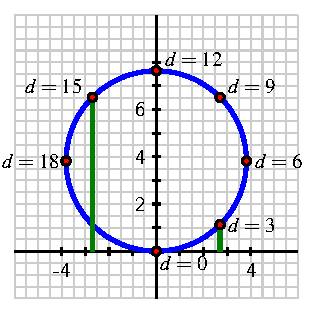
\includegraphics[width=3in]{traversing-first-example.pdf}
%\end{image}
%
%
%Note that we know the exact heights of certain points. Since the circle has circumference $C = 24$, we know that $24 = 2\pi r$ and therefore $r = \frac{12}{\pi} \approx 3.82$.  Hence, the point where $d = 6$ (located $1/4$ of the way along the circle) is at a height of $h = \frac{12}{\pi} \approx 3.82$.  Doubling this value, the point where $d = 12$ has height $h = \frac{24}{\pi} \approx 7.64$.  Other heights, such as those that correspond to $d = 3$ and $d = 15$ (identified on the figure by the green line segments) are not obvious from the circle's radius, but can be estimated from the grid in the figure above as $h \approx 1.1$ (for $d = 3$) and $h \approx 6.5$ (for $d = 15$).  Using all of these observations along with the symmetry of the circle, we can construct a table..
%
%\begin{center}
%$
%\begin{array}{ |c || c|  }
% \hline
% d & h\\
% \hline
% 0&0\\
% 3&1.1\\
% 6&3.82\\
% 9&6.5\\
% 12&7.64\\
% 15&6.5\\
% 18&3.82\\
% 21&1.1\\
% 24&0\\
% \hline
%\end{array}
%$
%\end{center}
%
%Moreover, if we now let the point continue traversing the circle, we observe that the $d$-values will increase accordingly, but the $h$-values will repeat according to the already-established pattern, resulting in the data in the table below.
%
%\begin{center}
%$
%\begin{array}{ |c || c|  }
% \hline
% d & h\\
% \hline
% 24&0\\
% 27&1.1\\
% 30&3.82\\
% 33&6.5\\
% 36&7.64\\
% 39&6.5\\
% 42&3.82\\
% 45&1.1\\
% 48&0\\
% \hline
%\end{array}
%$
%\end{center}
%
%It is apparent that each point on the circle corresponds to one and only one height, and thus we can view the height of a point as a function of the distance the point has traversed around the circle, say $h = f(d)$.  Using the data from the two tables and connecting the points in an intuitive way, we get the graph shown below
%
%\begin{image}
%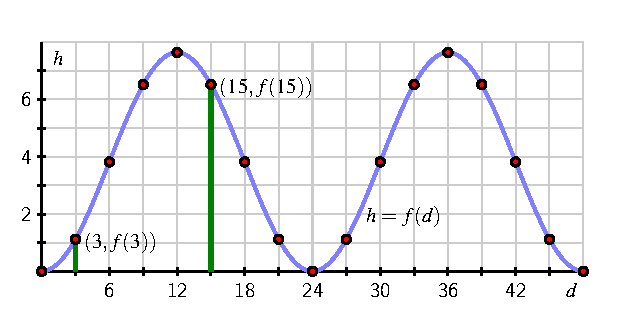
\includegraphics{traversing-first-example-graph.pdf}
%\end{image}
%
%% How do I transition from that example to talking about periodicity
%
%Notice that the graph above resembles the graph of the sine function. As it turns out, the sine function exhibits some of the same oscillatory behavior as $f$. This shared property turns out to be very important, especially when looking at functions that are related to circles. 
%
%\begin{definition}
%Let $f$ be a function whose domain and codomain % Have these been introduced?
%are each the set of all real numbers. We say that $f$ is \index{function ! periodic}\index{periodic function}\dfn{periodic} provided that there exists a real number $k$ such that $f(x + k) = f(x)$ for every possible choice of $x$. The smallest positive value $p$ for which $f(x + p) = f(x)$ for every choice of $x$ is called the \index{period}\dfn{period} of $f$.
%
%\end{definition}
%
%For our ferris wheel example above, the period is the circumference of the circle that generates the curve. In the graph, we see how the curve has completed one full cycle of behavior every 24 units, regardless of where we start on the curve.
%
%Two important periodic functions are the sine function, which you have seen, and the cosine function, which resembles the sine function. You will study these functions and learn about their relationship with circles in trigonometry.
%
%As a reminder, here is a graph of the sine function along with a table listing some of its values.
%
%\begin{image}
%\begin{tikzpicture}
%    \begin{axis}[ymin=-2, ymax=2,
%		   %xtick={-6.28318, -4.7123889, -3.14159, -1.5708, 1.5708, 3.14159, 4.7123889, 6.28318},
%    xticklabels={
%        $-\frac{3\pi}{2}$, $-\pi$, $\frac{\pi}{2}$, $0$,
%        $\frac{\pi}{2}$, $\pi$, $\frac{3\pi}{2}$, $2\pi$
%    }, ]
%        \addplot[samples=200]{sin(pi/4*deg(x))};
%    \end{axis}
%\end{tikzpicture}
%\end{image}
%
%\begin{center}
%$\arraycolsep=1.4pt\def\arraystretch{2.2}
%\begin{array}{ |c|c|  }
% \hline
% \multicolumn{2}{|c|}{\text{\normalfont Important Values of }y=\sin(x)} \\
%\hline
% \hline
% x & y\\
% \hline
%
% -\pi&\text{ }0\\
%
% -\frac{\pi}{2}&-1\\
%
% 0&\text{ }0\\
%
% \frac{\pi}{2}&\text{ }1\\
%
% \pi&\text{ }0\\
%
%\frac{3\pi}{2}&-1\\
%
% 2 \pi&\text{ }0\\
%\hline
%\end{array}
%$
%\end{center} 
%
%Notice that $\sin\left(-\frac{\pi}{2}\right) = -1$ and $\sin\left(\frac{3\pi}{2}\right) = -1$ as well. In fact, the sine function is periodic with period $2\pi$. 
%
%Now, here is a graph of the cosine function along with a table listing some of its values.
%
%\begin{image}
%\begin{tikzpicture}
%    \begin{axis}[ymin=-2, ymax=2,
%		   %xtick={-6.28318, -4.7123889, -3.14159, -1.5708, 1.5708, 3.14159, 4.7123889, 6.28318},
%    xticklabels={
%        $-\frac{3\pi}{2}$, $-\pi$, $\frac{\pi}{2}$, $0$,
%        $\frac{\pi}{2}$, $\pi$, $\frac{3\pi}{2}$, $2\pi$
%    }, ]
%        \addplot[samples=200]{cos(pi/4*deg(x))};
%    \end{axis}
%\end{tikzpicture}
%\end{image}
%
%\begin{center}
%$\arraycolsep=1.4pt\def\arraystretch{2.2}
%\begin{array}{ |c | c|  }
% \hline
% \multicolumn{2}{|c|}{\text{\normalfont Important Values of } y=\cos(x)} \\
%\hline
% \hline
% x & y\\
% \hline
%
% -\pi&-1\\
%
% -\frac{\pi}{2}&\text{ }0\\[2ex]
%
% 0&\text{ }1\\
%
% \frac{\pi}{2}&\text{ }0\\[2ex]
%
% \pi&-1\\
%
%\frac{3\pi}{2}&\text{ }0\\[2ex]
%
% 2 \pi&\text{ }1\\
%\hline
%\end{array}
%$
%\end{center} 
%
%Notice that $\cos\left(-\pi\right) = -1$ and $\cos\left(\pi\right) = -1$ as well. In fact, the cosine function is also periodic with period $2\pi$. 
% 


%\typeout{************************************************}
%\typeout{Odd and even functions}
%\typeout{************************************************}

\section{Odd and even functions}

Consider the two functions, $g(x) = x^3$ and $h(x) = x^2$, whose graphs are shown below.
\begin{image}
\begin{tikzpicture}
    \begin{axis}[title={$g(x) = x^3$}]
        \addplot[smooth]{x^3} node{$g(x) = x^3$};
    \end{axis}
\end{tikzpicture}

\begin{tikzpicture}
    \begin{axis}[title={$h(x) = x^2$}]
        \addplot[smooth]{x^2} node{$h(x)=x^2$};
    \end{axis}
\end{tikzpicture}
\end{image}

Note that the graph of $g$ seems to be symmetric about the origin, meaning that when we rotate the graph a half-turn, we get the same graph. Also, the graph of $h$ seems to be symmetric about the $y$-axis, meaning that when we flip the graph across the $y$-axis, we get the same graph. 

Let's first consider the case of $g$ by looking at a few test points. 


\begin{align*}
g(2) & = (2)^3 = 8\\
g(-2) & = (-2)^3 = -8\\
g(3) & = (3)^3 = 27\\ 
g(-3) & = (-3)^3 = -27
\end{align*}

We see that $(2,8)$, $(-2,8)$, $(3,27)$, and $(-3,-27)$ are points on the graph which indicates $g(x)$ is an odd function. We can check this for all point, showing that $(-x,-y)$ is on the graph whenever $(x,y)$ is.  In other words, we need to show $(-x,-y)$ satisfies the equation $y = x^3$ whenever $(x,y)$ does.  Substituting $(-x, -y)$ into the equation gives


$$g(-x) = (-x)^3= -x\cdot -x \cdot -x = -x^3 = -g(x)$$

 This shows that $g$ is an odd function.



\begin{exploration}
Consider the function $h$ defined by $h(x) = x^2$. We'll try to prove that $h$ is symmetric about the $y$-axis. 
\begin{enumerate}[label=\alph*.]
\item Assume $(x, y)$ is a generic point on the graph of $h$, so $y = x^2$. What point is symmetric to $(x, y)$ about the $y$-axis?
\item Show your answer to part a is on the graph of $h$ whenever $(x, y)$ is. Conclude that $h$ is symmetric about the $y$-axis. 
\end{enumerate}
\end{exploration}

Notice that to test an equation's graph for symmetry about the origin, we replaced $x$ and $y$ with $-x$ and $-y$, respectively.  Doing this substitution in the equation $y = f(x)$ results in $-y = f(-x)$.  Solving the latter equation for $y$ gives $y = -f(-x)$.  In order for this equation to be equivalent to the original equation $y=f(x)$ we need $-f(-x) = f(x)$, or, equivalently, $f(-x) = -f(x)$. In the exploration, you checked whether the graph of an equation was symmetric about the $y$-axis by replacing $x$ with $-x$ and checking to see if an equivalent equation results.  If we are graphing the equation $y=f(x)$, substituting $-x$ for $x$ results in the equation $y=f(-x)$.  In order for this equation to be equivalent to the original equation $y=f(x)$ we need $f(-x) = f(x)$. This leads us to the definition of an even function and an odd function.

\begin{definition}

A function $f$ is \dfn{even} if $f(-x) = f(x)$ for all $x$ in the domain of $f$. That is, if $(x,y)$ is a point of $f$, so is $(-x,y)$.



\end{definition}

\begin{definition}

A function $f$ is \dfn{odd} if $f(-x) = -f(x)$ for all $x$ in the domain of $f$. That is, if $(x,y)$ is a point of $f$, so is $(-x,-y)$.

\end{definition}

A function is even if and only if its graph is symmetric about the $y$-axis.  A function is odd if and only if its graph is symmetric about the origin.  

\begin{example}
Determine if the following functions are even, odd, or neither even nor odd using the definition of even and odd functions. 
\begin{enumerate}
\item $f(x) = \frac{5}{2 - x^2}$ 
\item $g(x) = \frac{5x}{2 - x^2}$ 
\item $h(x) = \frac{5x}{2 - x^3}$
\end{enumerate}
\end{example}


\begin{explanation}
The defintion of even and odd functions gives information about $f(-x)$, the first step in all these problems is to replace input $-x$ into the function and simplify.

\begin{enumerate}
\item Here, $f(x) = \frac{5}{2 - x^2}$. Inputting $-x$ into $f$, we find that

\begin{align*}
f(-x) & = \frac{5}{2 - (-x)^2}\\
f(-x) & = \frac{5}{2 - (-1 \cdot x)^2}\\
f(-x) & = \frac{5}{2 - (-1)^2 \cdot x^2}\\
f(-x) & = \frac{5}{2 - x^2},
\end{align*}

so $f(-x) = f(x)$. This shows that $f$ is \emph{even}. 

\item Here, $g(x) = \frac{5x}{2 - x^2}$. Inputting $-x$ into $g$, we find that

\begin{align*}
g(-x) & = \frac{5(-x)}{2 - (-x)^2}\\
g(-x) & = \frac{-5x}{2 - x^2}.
\end{align*}

It doesn't appear that $g(-x)$ is equal to $g(x)$. To prove this, we check with an $x$ value. After some trial and error, we see that $g(1) = 5$ whereas $g(-1) = -5$. This proves that $g$ is not even, but it doesn't rule out the possibility that $g$ is odd. (Why not?) To check if $g$ is odd, we compare $g(-x)$ with $-g(x)$:

\begin{align*}
-g(x) & = -\frac{5x}{2 - x^2} \\
-g(x) & = \frac{-5x}{2 - x^2} \\
-g(x) & = g(-x).
\end{align*}
Since $-g(x) = g(-x)$, $g$ is \emph{odd}.

\item Here, $h(x) = \frac{5x}{2 - x^3}$. Inputting $-x$ into $h$, we find that 

\begin{align*}
h(-x) & = \frac{5(-x)}{2 - (-x)^3} \\
h(-x) & = \frac{-5x}{2 + x^3}.
\end{align*}

Once again, $h(-x)$ doesn't appear to be equal to $h(x)$. We check with an $x$ value. For example, $h(1) = 5$, but $h(-1) = -\frac{5}{3}$. This proves that $h$ is not even and it also shows $h$ is not odd. You may be wondering how we konw that $h$ is not odd.  Recall that when $h$ is odd, then if $(x_1,y_1)$ is a point on $h$, then $(-x_1,-y_1)$ must also be a point on $h$.  But that would mean that for $h$ to be odd, $h(-1)=-h(1)$.  But $-h(1)=-5$ and $h(-1)= -\frac{5}{3} \neq -5$.

\end{enumerate}
\end{explanation}

\section{Completing the Graph of Even or Odd Functions}

If we know a function is either even or odd, we can determine one half of the graph or function values if we are giving the other half.  This is because we know that:
\begin{itemize}
\item If a function is \textbf{even} and the point $(x_1,y_1)$ is on the function graph, then the point $(-x_1,y_1)$ is also on the function graph.
\item If a function is \textbf{odd} and the point $(x_1,y_1)$ is on the function graph, then the point $(-x_1,-y_1)$ is also on the function graph.
\end{itemize}

Try the two examples below and then compare your work with the solution. 


\begin{example} \textit{Even} \\

Half of the graph of $y = K(t)$ is displayed below.   If $K(t)$ is an even function, then think of what the other half of the graph would look like.



\begin{image}
\begin{tikzpicture}
     \begin{axis}[
                domain=-10:10, ymax=10, xmax=10, ymin=-10, xmin=-10,
                axis lines =center, xlabel=$t$, ylabel=${y=K(t)}$,
                ytick={-10,-8,-6,-4,-2,2,4,6,8,10},
                xtick={-10,-8,-6,-4,-2,2,4,6,8,10},
                ticklabel style={font=\scriptsize},
                every axis y label/.style={at=(current axis.above origin),anchor=south},
                every axis x label/.style={at=(current axis.right of origin),anchor=west},
                axis on top,
                ]

        
        %\addplot [draw=penColor, very thick, smooth, domain=(-7.5:3), <->] {1/(x-3) + 2};
        \addplot [draw=penColor, very thick, smooth, domain=(3:6), <-] {1/(x-3) + 2};
        \addplot [draw=penColor, very thick, smooth, domain=(6:8), ->] {2*x-14};

        \addplot [line width=1, gray, dashed,samples=100,domain=(-9:9)] ({3},{x});
        %\addplot [line width=1, gray, dashed,samples=100,domain=(-9:4)] ({x},{2});

        %\addplot[color=penColor,fill=penColor,only marks,mark=*] coordinates{(-6,5)};
        %\addplot[color=penColor,fill=white,only marks,mark=*] coordinates{(-6,1.88)};
        \addplot[color=penColor,fill=penColor,only marks,mark=*] coordinates{(6,2.33)};
        \addplot[color=penColor,fill=white,only marks,mark=*] coordinates{(6,-2)};

    \end{axis}



\end{tikzpicture}
\end{image}

Visualize what the full graph looks like, then click the arrow to compare with the solution below.

%\begin{expandable}

\begin{explanation}

To sketch our graph, we’ll use the following fact: If a function is \textbf{even} and the point $(x_1,y_1)$ is on the function graph, then the point $(-x_1,y_1)$ is also on the function graph.
First, let’s look at the linear portion of the graph. This is a line with a hole at $(6,-2)$ and an $x$-intercept at $(7,0)$. This tells us that we have a hole at $(-6,-2)$ and an $x$-intercept at $(-7,0)$. We then draw a line from $(-6,-2)$, through the point $(-7,0)$. Next, we see a point at approximately $(6,2.25)$ so we plot the point $(-6,2.25)$. There’s a vertical asymptote at $x=3$ so we’ll sketch the vertical asymptote $x=-3$. Last, we’ll sketch the function from $(6,2.25)$, curving up toward the vertical asymptote $x=-3$.

\begin{image}
\begin{tikzpicture}
     \begin{axis}[
                domain=-10:10, ymax=10, xmax=10, ymin=-10, xmin=-10,
                axis lines =center, xlabel=$t$, ylabel=${y=K(t)}$,
                ytick={-10,-8,-6,-4,-2,2,4,6,8,10},
                xtick={-10,-8,-6,-4,-2,2,4,6,8,10},
                ticklabel style={font=\scriptsize},
                every axis y label/.style={at=(current axis.above origin),anchor=south},
                every axis x label/.style={at=(current axis.right of origin),anchor=west},
                axis on top,
                ]

        
        \addplot [draw=penColor, very thick, smooth, samples=300, domain=(-6:-3.15), ->] {-1/(x+3) + 2};
        \addplot [draw=penColor, very thick, smooth, samples=300, domain=(-8:-6), <-] {-2*x-14};
        \addplot [draw=penColor, very thick, smooth, samples=300, domain=(3.15:6), <-] {1/(x-3) + 2};
        \addplot [draw=penColor, very thick, smooth, samples=300, domain=(6:8), ->] {2*x-14};

        \addplot [line width=1, gray, dashed,samples=100,domain=(-9:9)] ({3},{x});
        \addplot [line width=1, gray, dashed,samples=100,domain=(-9:9)] ({-3},{x});

        \addplot[color=penColor,fill=penColor,only marks,mark=*] coordinates{(-6,2.33)};
        \addplot[color=penColor,fill=white,only marks,mark=*] coordinates{(-6,-2)};
        \addplot[color=penColor,fill=penColor,only marks,mark=*] coordinates{(6,2.33)};
        \addplot[color=penColor,fill=white,only marks,mark=*] coordinates{(6,-2)};

    \end{axis}



\end{tikzpicture}
\end{image}

\end{explanation}

%\end{expandable}

\end{example}


\begin{example} \textit{Odd} \\

Half of the graph of $y = M(t)$ is displayed below.   If $M(t)$ is an odd function, then think of what the other half of the graph would look like.



\begin{image}
\begin{tikzpicture}
     \begin{axis}[
                domain=-10:10, ymax=10, xmax=10, ymin=-10, xmin=-10,
                axis lines =center, xlabel=$t$, ylabel=${y=M(t)}$,
                ytick={-10,-8,-6,-4,-2,2,4,6,8,10},
                xtick={-10,-8,-6,-4,-2,2,4,6,8,10},
                ticklabel style={font=\scriptsize},
                every axis y label/.style={at=(current axis.above origin),anchor=south},
                every axis x label/.style={at=(current axis.right of origin),anchor=west},
                axis on top,
                ]

        
        %\addplot [draw=penColor, very thick, smooth, domain=(-7.5:3), <->] {1/(x-3) + 2};
        \addplot [draw=penColor, very thick, smooth, domain=(3:6), <-] {1/(x-3) + 2};
        \addplot [draw=penColor, very thick, smooth, domain=(6:8), ->] {2*x-14};

        \addplot [line width=1, gray, dashed,samples=100,domain=(-9:9)] ({3},{x});
        %\addplot [line width=1, gray, dashed,samples=100,domain=(-9:4)] ({x},{2});

        %\addplot[color=penColor,fill=penColor,only marks,mark=*] coordinates{(-6,5)};
        %\addplot[color=penColor,fill=white,only marks,mark=*] coordinates{(-6,1.88)};
        \addplot[color=penColor,fill=penColor,only marks,mark=*] coordinates{(6,2.33)};
        \addplot[color=penColor,fill=white,only marks,mark=*] coordinates{(6,-2)};

    \end{axis}



\end{tikzpicture}
\end{image}

Visualize what the full graph looks like, then click the arrow to compare with the solution below.


%\begin{expandable}

\begin{explanation}

If a function is \textbf{odd} and the point $(x_1,y_1)$ is on the function graph, then the point $(-x_1,-y_1)$ is also on the function graph. First, let’s look at the linear portion of the graph. This is a line with a hole at $(6,-2)$ and an $x$-intercept at $(7,0)$. This tells us that we have a hole at $(-6,2)$ and an $x$-intercept at $(-7,0)$. We then draw a line from $(-6,2)$, through the point $(-7,0)$. Next, we see a point at approximately $(6,2.25)$ so we plot the point $(-6,-2.25)$. There’s a vertical asymptote at $x=3$ so we’ll sketch the vertical asymptote $x=-3$. Last, we’ll sketch the function from $(-6,-2.25)$, curving up toward the vertical asymptote $x=-3$.

\begin{image}
\begin{tikzpicture}
     \begin{axis}[
                domain=-10:10, ymax=10, xmax=10, ymin=-10, xmin=-10,
                axis lines =center, xlabel=$t$, ylabel=${y=M(t)}$,
                ytick={-10,-8,-6,-4,-2,2,4,6,8,10},
                xtick={-10,-8,-6,-4,-2,2,4,6,8,10},
                ticklabel style={font=\scriptsize},
                every axis y label/.style={at=(current axis.above origin),anchor=south},
                every axis x label/.style={at=(current axis.right of origin),anchor=west},
                axis on top,
                ]

        
        \addplot [draw=penColor, very thick, smooth, samples=300, domain=(-6:-3.15), ->] {1/(x+3) - 2};
        \addplot [draw=penColor, very thick, smooth, samples=300, domain=(-8:-6), <-] {2*x+14};
        \addplot [draw=penColor, very thick, smooth, samples=300, domain=(3.15:6), <-] {1/(x-3) + 2};
        \addplot [draw=penColor, very thick, smooth, samples=300, domain=(6:8), ->] {2*x-14};

        \addplot [line width=1, gray, dashed,samples=100,domain=(-9:9)] ({3},{x});
        \addplot [line width=1, gray, dashed,samples=100,domain=(-9:9)] ({-3},{x});

        \addplot[color=penColor,fill=penColor,only marks,mark=*] coordinates{(-6,-2.33)};
        \addplot[color=penColor,fill=white,only marks,mark=*] coordinates{(-6,2)};
        \addplot[color=penColor,fill=penColor,only marks,mark=*] coordinates{(6,2.33)};
        \addplot[color=penColor,fill=white,only marks,mark=*] coordinates{(6,-2)};

    \end{axis}



\end{tikzpicture}
\end{image}

\end{explanation}
%\end{expandable}


\end{example}

\begin{summary}\begin{itemize}
%\item For a function $f$ defined on the real numbers, we say $f$ is periodic if there exists some $k$ such that
%\begin{equation*}
%f(x + k) = f(x)
%\end{equation*}
%for all possible choices of $x$. The smallest value of $k$ for which $f(x + k) = f(x)$ for all possible choices of $x$ is called the period of $f$.
\item A function $f$ is called
\begin{itemize}
\item even if $f(-x) = f(x)$ for all possible choices of $x$. Even functions are symmetric about the $y$-axis. 
\item odd if $f(-x) = -f(x)$ for all possible choices of $x$. Odd functions are symmetric about the origin. 
\end{itemize}
\end{itemize}\end{summary}


\end{document}
